\documentclass[conference]{IEEEtran}
\IEEEoverridecommandlockouts

\usepackage{cite}
\usepackage{amsmath,amssymb,amsfonts}
\usepackage{mathtools}
\usepackage{algorithmic}
\usepackage{graphicx}
\usepackage{textcomp}
\usepackage{xcolor}
\usepackage{textcomp}
\usepackage{float}
\usepackage{array}
\usepackage{siunitx}
\usepackage{tabularx}
\usepackage{listings}
\usepackage{accents}
\usepackage{nicematrix,tikz}
\usepackage{setspace}
\usepackage[colorlinks=false]{hyperref}
\def\BibTeX{{\rm B\kern-.05em{\sc i\kern-.025em b}\kern-.08em
    T\kern-.1667em\lower.7ex\hbox{E}\kern-.125emX}}

\setlength{\parindent}{0pt}

% Define the custom column type Y
\newcolumntype{Y}{>{\centering\arraybackslash} m{1cm}}

\definecolor{codeblue}{rgb}{0.2,0.2,0.6}
\definecolor{codegreen}{rgb}{0.133,0.545,0.133}
\definecolor{codegray}{rgb}{0.5,0.5,0.5}
\definecolor{codepurple}{rgb}{0.58,0,0.82}
\definecolor{backcolour}{rgb}{0.95,0.95,0.92}

\lstdefinestyle{mystyle}{
    backgroundcolor=\color{backcolour},
    commentstyle=\color{codegreen},
    keywordstyle=\color{codeblue},
    numberstyle=\tiny\color{codegray},
    stringstyle=\color{codepurple},
    basicstyle=\ttfamily\scriptsize,
    breakatwhitespace=false,
    breaklines=true,
    captionpos=b,
    keepspaces=true,
    numbers=none,
    numbersep=5pt,
    showspaces=false,
    showstringspaces=false,
    showtabs=false,
    tabsize=2
}
\lstset{style=mystyle}

\title{Robotics and Mechatronics\\
{\LARGE Mini Project Two}
}

\author{\IEEEauthorblockN{Mohammad Montazeri}
    \IEEEauthorblockA{\textit{School of Mechanical Engineering} \\
        \textit{College of Engineering, University of Tehran}\\
        Tehran, Iran; 810699269 \\
        mohammadmontazeri@ut.ac.ir}
}

\begin{document}
\maketitle

\begin{abstract}
    This mini project is designed to address the kinematics and dynamics of robotic arms using MATLAB and \textit{Simscape} environment. The given case study in this project is the known \textit{Scara} robotic arm.
\end{abstract}

\begin{IEEEkeywords}
    Scara, dynamics, kinematics, simulation, jacobian
\end{IEEEkeywords}

\section{Introduction}
SCARA (Selective Compliance Articulated Robot Arm) robots, known for their precise X-Y plane movements, excel in material handling tasks and assembly work. Their versatility and cost-effectiveness make them popular in manufacturing environments. This report discusses a specific kind of this robot, as a valuable asset in various industries.

\section{Denavit-Hartenberg Parameters}
According to the vectors shown in Figure~\ref{fig:scara}, the following D-H
table can be drawn.

\begin{table}[htbp]
    \caption{The D-H parameters of SCARA robot}
    \def\arraystretch{1.21}
    \begin{center}
        \begin{tabular}{|Y|Y|Y|Y|Y|Y|}
            \hline
            $i$ & $a_i$ & $b_i$  & $\alpha_i$  & $\theta_i$ & $q_i^{initial}$ \\
            \hline
            1   & 0     & $b_1$  & $90^\circ$  & 0          & 800mm           \\
            \hline
            2   & 400   & 257.7  & 0           & $\theta_2$ & 0               \\
            \hline
            3   & 250   & 0      & 0           & $\theta_3$ & $90^\circ$      \\
            \hline
            4   & 0     & $-b_4$ & $180^\circ$ & 0          & 100mm           \\
            \hline
        \end{tabular}
    \end{center}
\end{table}

\begin{figure}[htbp]
    \centerline{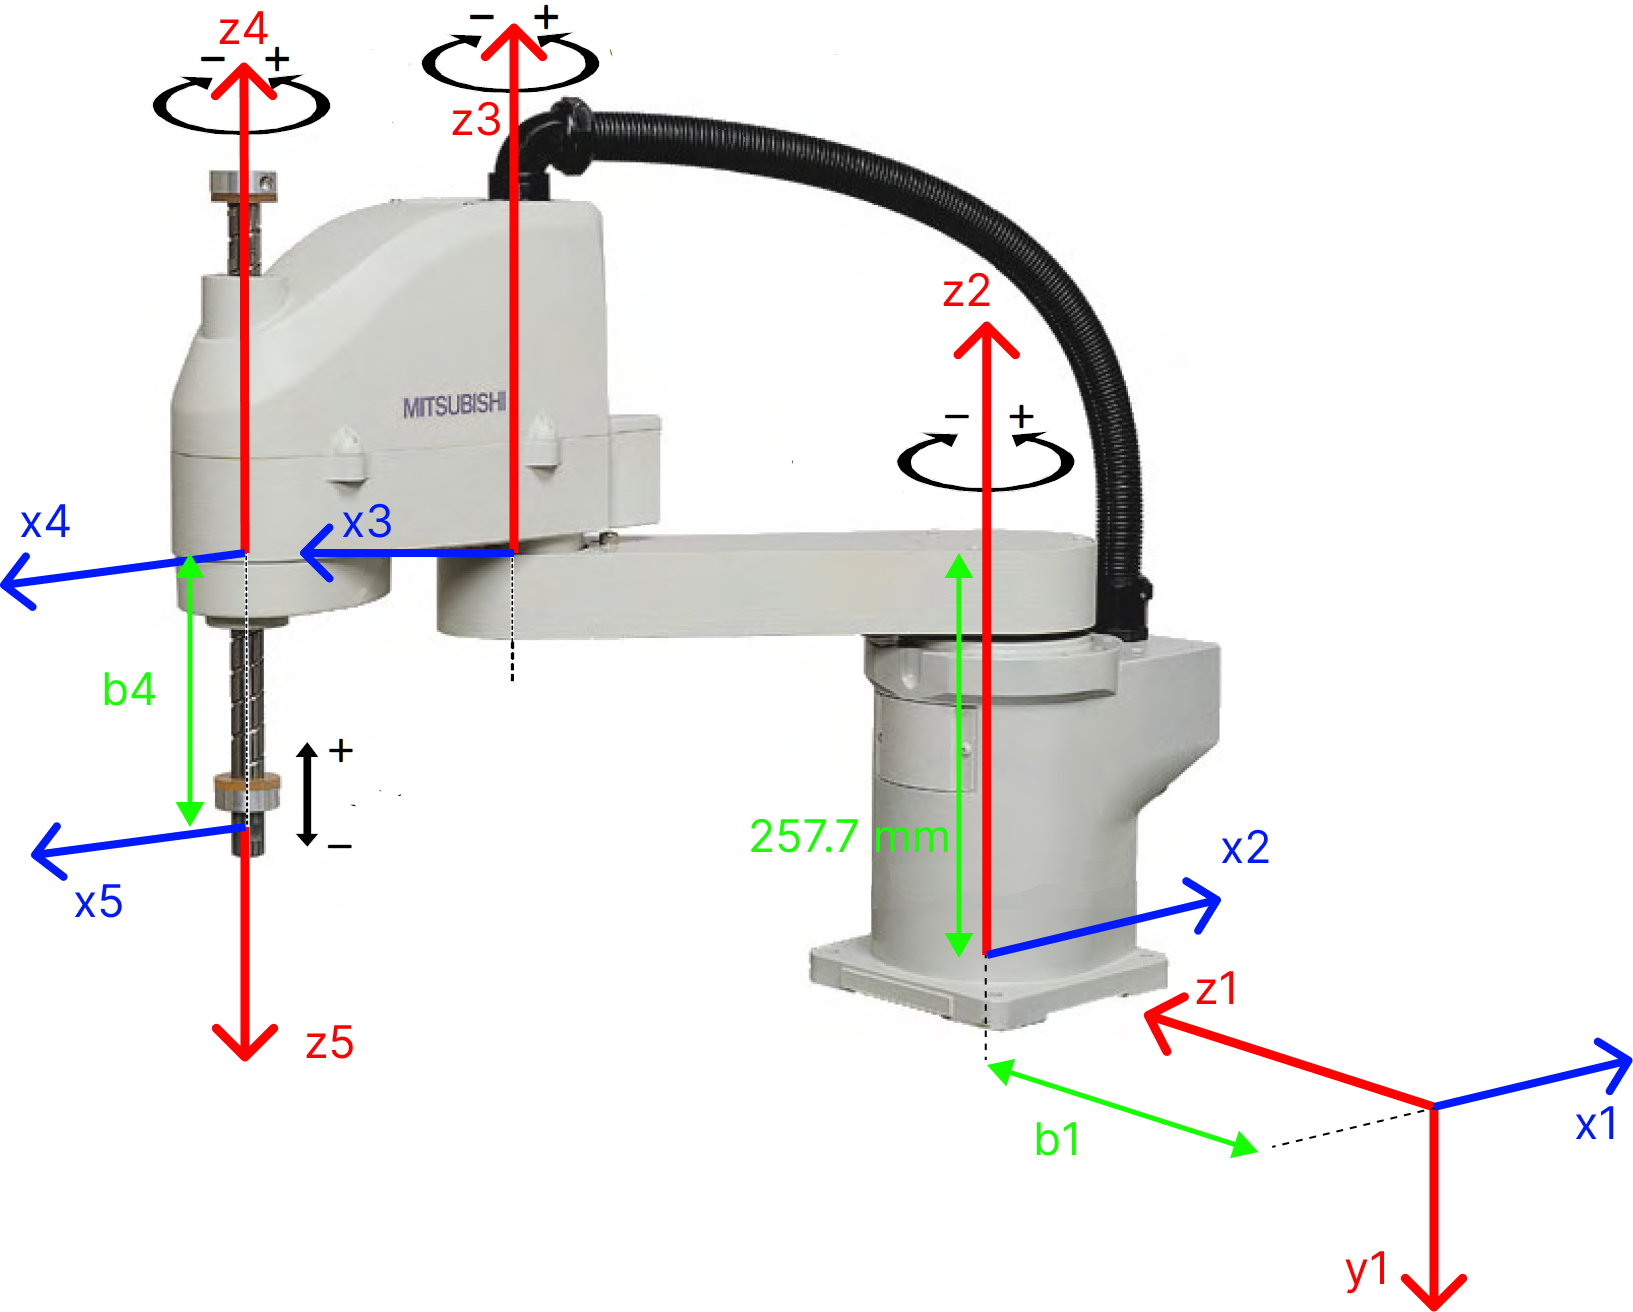
\includegraphics[width=0.4\textwidth]{figures/SCARA.png}}
    \caption{SCARA robot marked up with D-H vectors. Raw image courtesy of Wikipedia\cite{b3}.}
    \label{fig:scara}
\end{figure}

\section{Forward Kinematic Problem}
\begin{align}
    Q_i =                       & \begin{bmatrix}
                                      \cos \theta_i & - \cos \alpha_i \sin \theta_i & \sin \alpha_i \sin \theta_i   \\
                                      \sin \theta_i & \cos \alpha_i \cos \theta_i   & - \sin \alpha_i \cos \theta_i \\
                                      0             & \sin \alpha_i                 & \cos \alpha_i
                                  \end{bmatrix} \label{eq:Q}                                                             \\
    \vec{\mathbf{a_i}} =        & \begin{bmatrix}
                                      a_i \cos \theta_i \\
                                      a_i \sin \theta_i \\
                                      b_i
                                  \end{bmatrix} \hspace{50px} Q=Q_1 Q_2 Q_3 Q_4 \label{eq:a}                                                                                \\
    \vec{\mathbf{\mathit{P}}} = & \begin{bmatrix}
                                      x_w \\
                                      y_w \\
                                      z_w
                                  \end{bmatrix} = \mathbf{a_1} + Q_1 \mathbf{a_2} + Q_1 Q_2 \mathbf{a_3} + Q_1 Q_2 Q_3 \mathbf{a_4} \label{eq:P}                            \\
    T =                         & \begin{bmatrix}
                                      Q                  & \vec{\mathbf{\mathit{P}}} \\
                                      \vec{0}_{1\times3} & 1
                                  \end{bmatrix} \hspace{10px} \phi = \arccos\left(\frac{tr(Q) - 1}{2}\right) \hspace{10px} \vec{e} = \frac{vect(Q)}{\sin \phi} \label{eq:T}
\end{align}

Having D-H variables of the robot, all parameters above can be calculated via MATLAB. Here's its final results:
\begin{small}
    \begin{align*}
         & x = 250.0\,\cos\left(\theta _{2}+\theta _{3}\right)+400.0\,\cos\left(\theta _{2}\right)                                              \\
         & y = b_{4}+1.5\,{10}^{-14}\,\sin\left(\theta _{2}+\theta _{3}\right)+2.4\,{10}^{-14}\,\sin\left(\theta _{2}\right)-257.7              \\
         & z = b_{1}-6.1\,{10}^{-17}\,b_{4}+250.0\,\sin\left(\theta _{2}+\theta _{3}\right)+400.0\,\sin\left(\theta _{2}\right)+1.6\,{10}^{-14}
    \end{align*}
\end{small}

Omitting the terms close to zero (of order $10^{-14}$ or lower), we gain the same values as analytical solution, according to the chosen $x_1, y_1, y_1$ axes shown in Figure~\ref{fig:scara}.
\begin{align}
    x    & = 400 \cos \theta_2 + 250 \cos (\theta_2 + \theta_3)    \label{eq:x}    \\
    y    & = - (257.7 - b_4)                                        \label{eq:y}   \\
    z    & = b_1 + 400 \sin \theta_2 + 250 \sin (\theta_2 + \theta_3) \label{eq:z} \\
    \phi & = \theta_2 + \theta_3 \label{eq:phi1}
\end{align}

The rotation matrix after being filtered by removing the terms close to zero, can be shown as below. Using equation \ref{eq:T}, the final rotation angle can also be derived from the obtained $Q$.
\begin{gather}
    Q = \begin{bmatrix}
        \cos\left(\theta _{2}+\theta _{3}\right) & \sin\left(\theta _{2}+\theta _{3}\right)      & 0.0 \\
        0.0                                      & 0.0                                           & 1.0 \\
        \sin\left(\theta _{2}+\theta _{3}\right) & 1.0\,\cos\left(\theta _{2}+\theta _{3}\right) & 0
    \end{bmatrix} \\
    \phi = \cos^{-1} \left(0.5 \cos \left(\theta_2 + \theta_3\right) - 0.5\right) \label{eq:phi2}
\end{gather}

The overall homogenous rotation-displacement transformation matrix with the initial conditions\footnote{$\, \theta_2=0, \quad \theta_3=90^\circ, \quad b_1=800mm, \quad b_4=100mm$} chosen for this problem is calculated as:
\begin{align*}
    \left(\begin{array}{cccc} 0 & 1 & 0 & 400\\ 0 & 0 & 1 & -158\\ 1 & 0 & 0 & 1050\\ 0 & 0 & 0 & 1 \end{array}\right)
\end{align*}

In another simpler representation, the following position and orientation is achieved with the mentioned initial conditions.
\begin{align*}
    x = 400 mm \quad y = -157.7 mm \quad z = 1050 mm \quad \phi = 90^\circ
\end{align*}
\vspace{10px}

\section{Inverse kinematic Problem}
Playing with equations \ref{eq:x} to \ref{eq:phi1} we can find the IKP equations as below. Having the task-space parameters $x, y, z \, \& \, \phi$, we can calculate joint-space parameters $b_1, b_4, \theta_2 \, \& \, \theta_3$ as:
% \begin{align*}
%     \cos \phi = 0.5 \left(\cos (\theta_2 + \theta_3) - 1\right) \rightarrow \theta_2 + \theta_3 = \arccos \left(2\cos \phi + 1\right)                                                 \\
%     b_4 = y + 257.7                                                                                                                                                                   \\
%     x = 400 \cos \theta_2 + 250 \cos \left(\arccos \left(2\cos \phi + 1\right)\right) = 400 \cos \theta_2 + 250 \left(2\cos \phi + 1\right) = 400 \cos \theta_2 + 500 \cos \phi + 250 \\
%     z = b_1 + 400 \sin \theta_2 + 250 \sin \left(\arccos \left(2\cos \phi + 1\right)\right) \rightarrow                                                                               \\
%     (x - 400 \cos \theta_2)^2 + (z - 400 \cos \theta_2 - b_1)^2 = 250^2 \left(\cos^2 (\theta_2 + \theta_3) + \sin^2 (\theta_2 + \theta_3) \right) = 62500                             \\
% \end{align*}

\begin{align}
     & \rightarrow b_4         = y + 257.7                                                                                       \\
     & x           = 400 \cos \theta_2 + 250 \cos \phi \,\, , \,\, z         = b_1 + 400 \sin \theta_2 + 250 \sin \phi \nonumber \\
     & \rightarrow \theta_2 = \arccos \left(\frac{x - 250 \cos \phi}{400}\right)                                                 \\
     & \rightarrow b_1 = z - 400 \sin \theta_2 - 250 \sin \phi                                                                   \\
     & \rightarrow \theta_3    = \phi - \theta_2
\end{align}

With a glance of what's achieved, it can be concluded that there's always a unique answer for $b_4$, while the \textit{arccos} term in $\theta_2$ results two answers, leading to two answers for each of $\theta_2, \theta_3$ and $b_1$.
\begin{large}
    \begin{align*}
         & Answers \longrightarrow
        \begin{cases}
            \theta_2 ^+ \longrightarrow\theta_4 ^+ \longrightarrow b_1^+ \longrightarrow b_4 \\[20pt]
            \theta_2 ^- \longrightarrow\theta_1 ^- \longrightarrow b_1^- \longrightarrow b_4
        \end{cases}
    \end{align*}
\end{large}
\vspace{10px}

\section{Jacobian Matrix}
Since the first and the last joints are prismatic, we'd have
\begin{align}
    \undertilde{\mathcal{J}} = \begin{bmatrix}
                                   \vec{O}   & \vec{e_2}                  & \vec{e_3}                  & \vec{O}   \\
                                   \vec{e_1} & \vec{e_2} \times \vec{r_2} & \vec{e_3} \times \vec{r_3} & \vec{e_4} \\
                               \end{bmatrix}
\end{align}

However, since we're dealing with a 4-DoF robot, its Jacobian matrix must have a square $(4\times4)$ shape. This robot is meant to access 3 positional ($x, y, z$) and one angular ($\phi$) degrees of freedom. Thus the first row of the mentioned matrix will be reduced to
\begin{align}
    \undertilde{\mathcal{J}} = \begin{bmatrix}
                                   0         & 1                          & 1                          & 0         \\
                                   \vec{e_1} & \vec{e_2} \times \vec{r_2} & \vec{e_3} \times \vec{r_3} & \vec{e_4} \\
                               \end{bmatrix}_{4\times4}
\end{align}

Deriving the Jacobian in the first joint frame requires calculating each $e_i$ and $r_i$ in the first frame. That can be done using the following transformations.

\begin{scriptsize}
    \begin{align*}
        \left[\vec{a_1}\right]_1 = \begin{bmatrix}
                                       0 \\
                                       0 \\
                                       b_1
                                   \end{bmatrix}
        \, \left[\vec{a_2}\right]_2 = \begin{bmatrix}
                                          400 \cos \theta_2 \\
                                          400 \sin \theta_2 \\
                                          257.7
                                      \end{bmatrix}
        \, \left[\vec{a_3}\right]_3 = \begin{bmatrix}
                                          250 \cos \theta_3 \\
                                          250 \sin \theta_3 \\
                                          0
                                      \end{bmatrix}
        \, \left[\vec{a_4}\right]_4 = \begin{bmatrix}
                                          0 \\
                                          0 \\
                                          -b_4
                                      \end{bmatrix}
    \end{align*}
\end{scriptsize}

\begin{align*}
     & \left[\vec{e_2}\right]_1 = \undertilde{Q}_1 \left[\vec{e_2}\right]_2                                       \hspace{17px}
    \left[\vec{e_3}\right]_1 = \undertilde{Q}_1 \undertilde{Q}_2 \left[\vec{e_3}\right]_3                       \hspace{17px}
    \left[\vec{e_4}\right]_1 = \undertilde{Q}_1 \undertilde{Q}_2 \undertilde{Q}_3 \left[\vec{e_4}\right]_4                                               \\
     & \left[\vec{a_2}\right]_1 = \undertilde{Q}_1 \left[\vec{a_2}\right]_2                                       \hspace{16px}
    \left[\vec{a_3}\right]_1 = \undertilde{Q}_1 \undertilde{Q}_2 \left[\vec{a_3}\right]_3                       \hspace{16px}
    \left[\vec{a_4}\right]_1 = \undertilde{Q}_1 \undertilde{Q}_2 \undertilde{Q}_3 \left[\vec{a_4}\right]_4                                               \\
     & \left[\vec{r_2}\right]_1 = \left[\vec{a_2}\right]_1 + \left[\vec{a_3}\right]_1 + \left[\vec{a_4}\right]_1  \hspace{9px}
    \left[\vec{r_3}\right]_1 = \left[\vec{a_3}\right]_1 + \left[\vec{a_4}\right]_1                              \hspace{9px}
    \left[\vec{r_4}\right]_1 = \left[\vec{a_4}\right]_1                                                                                                  \\
     & \left[\vec{r_1}\right]_1 = \left[\vec{a_1}\right]_1 + \left[\vec{a_2}\right]_1 + \left[\vec{a_3}\right]_1 + \left[\vec{a_4}\right]_1 \label{eq:r}
\end{align*}

After doing the math via MATLAB and erasing the negligible terms\footnote{\, terms of order $10^{-14}$ or less, caused due to the computational errors which have occurred in the calculation process.}, here's the final result:
\begin{small}
    \begin{align*}
        \mathbf{J} = \begin{bmatrix}
                         0 & 1                                                                            & 1                                            & 0  \\
                         0 & -250\sin\left(\theta _{2}+\theta _{3}\right)-400\sin\left(\theta _{2}\right) & -250\sin\left(\theta _{2}+\theta _{3}\right) & 0  \\
                         0 & 0                                                                            & 0                                            & -1 \\
                         1 & 250\cos\left(\theta _{2}+\theta _{3}\right)+400\cos\left(\theta _{2}\right)  & 250\cos\left(\theta _{2}+\theta _{3}\right)  & 0
                     \end{bmatrix}
    \end{align*}
\end{small}

\section{Dynamic Model}
To use the Euler-Lagrange method, we need to find the kinetic energy ($T$) and potential energy ($V$) of the system.

\subsection{Kinetic Energy}
For each link, the kinetic energy is a combination of translational and rotational kinetic energy.
\begin{equation} \Large
    T = \sum_{1}^{4} \left(\frac{1}{2} \, m_i \, \dot{\vec{c}}_i^{\,T} \, \dot{\vec{c}}_i + \frac{1}{2} \, \vec{\omega}_i^T \, \mathbf{I}_i \, \vec{c}_i\right)
\end{equation}
where
\begin{itemize}
    \item $m_i$ is the mass of the $i$-th link.
    \item $\dot{\mathbf{c}}_i^{T}$ is the linear velocity of the center of mass of the $i$-th link.
    \item $\boldsymbol{\omega}_i$ is the angular velocity of the $i$-th link.
    \item $\mathbf{I}_i$ is the inertia tensor of the $i$-th link.
\end{itemize}


\subsection{Potential Energy}
The potential energy is due to gravity:
\begin{equation} \Large
    V = \sum_{1}^{4} \left(m_i g h_i\right)
\end{equation}
where $h_i$ is the height of the center of mass of the $i$-th link. It must be reminded that the obtained potential energy is not going to be directly used in this procedure, rather, its derivatives will be of use (see equation \ref{eq:L}). Thus, gravitational potential energy of links with no height alternation, which would be constant along any movement of the robot, will vanish after differentiation. Therefore, we are allowed to ignore them from the very beginning.

It can be put as by taking the ground level at $O_4$, we would only have the potential energy of the last (prismatic) link. That's because the centers of mass of the other links always have a constant height, invariant of any degree of freedom of the system. In other words, their height wouldn't change and since the potential energy terms are
used after differentiation, these constant values would be omitted. Accordingly, we only calculate the term related to the forth joint.

\begin{align}
    V = U_{g_4} = m_4 g h_4 = - 0.15 \times 9.81 \times b_4
\end{align}


\subsection{Euler-Lagrange Equation}
The Lagrangian is defined as:
\begin{equation} \Large
    \mathcal{L} = T - V
\end{equation}

Using the Euler-Lagrange equation for each generalized coordinate ($q_i$):
\begin{equation} \Large
    \frac{d}{dt} \left( \frac{\partial \mathcal{L}}{\partial \dot{q}_i} \right) - \frac{\partial \mathcal{L}}{\partial q_i} = \tau_i \label{eq:L}
\end{equation}
where $\tau_i$ represents the generalized forces/torques. \\

Computing these derivatives for each DoF ($q_i$) will yield the dynamic equations of motion for the SCARA robot. All this procedure is handled via \textit{Matlab} in a file called \texttt{torques\_using\_model.m} which accompanies this report file. Its results are also plotted and compared with the \textit{later-explained} simulation results via \texttt{plotting\_results.m} whose figures are attached in the Results section. It must also be mentioned that the following equations have a fundamental influence on the algorithm used to solve the dynamic model.
\begin{gather}
    [\mathrm{CoM}]_{DH}=T \, [\mathrm{CoM}]_{\text{link}} \\
    [I]_{DH}=Q \, [I]_{\text{link}} \, Q^{-1} \\
    T=\left(\begin{array}{ll}
            Q & b \\
            0 & 1
        \end{array}\right)
\end{gather}

\subsection{Simulation}
Along with this report comes a series of \textit{STL}, \textit{Simulink} and \textit{Matlab} files which together carry the burden of simulating this robot in \textit{Simscape} environment of \textit{Matlab}. For this matter, the STL files first need to be imported in \texttt{my\_second\_part\_R2018b.slx} for precise representation of the robot along its movement. After that, the input variables of the system must be given to the model. Therefore, a subsystem (Figure~\ref{fig:sub}) is added to the simulink file which imports inputs of the system. These inputs include each of the joint-space parameters ($b_1, b_4, \theta_2, \theta_3$) and their first 2 derivatives.\footnote{In other words, the position/orientation, velocity and acceleration of each joint.} To provide these variables, first the matlab codes must be run, so that the mentioned variables get saved in the workspace. It's suggested to run \texttt{parameters.m}, \texttt{torques\_using\_model.m}, \texttt{motions\_for\_simulink.m} and \texttt{my\_second\_part\_R2018b.slx} sequentially. It's also worth mentioning that importing the inputs could have been handled in both of the two ways explained below; while both of them are implemented in the provided Simulink file, the latter is currently used and the first method is commented out for now.
\begin{enumerate}
    \item \textbf{Importing the pre-derivated timeseries}: In the \texttt{motions\_for\_simulink.m} file, along with each $100001$-sample position/orientation variable, its first two derivatives are also calculated and available. We can directly import all of them into simscape.
    \item \textbf{Derivating using simulink}: It's also an option to only import the basic joint-space variables and use \textit{Simulink-PS Converter} block to find their derivates numerically via \textit{Input Handling} tab of the block.
\end{enumerate}
Using the combination of mentioned files, a smooth 4-5-6-7 trajectory planing pick-and-place is modeled whose initial and final situations are shown in Figure~\ref{fig:simulation}. It's worth mentioning that the initial and final conditions of the simulation is different from those of analytical solution and are defined as:
\begin{align*}
     & \theta_{init}^{sim} = [0, 0, 0, 0]                                     \\
     & \theta_{fin}^{sim} = \theta_{init}^{sim} + [0.5, \pi/3, -\pi/6, -0.05]
\end{align*}

After all, the output of the simulation, which is the collection of joint-space forces and torques, is both plotted and passed to the Matlab workspace for further comparison of the results. Figure~\ref{fig:sim_res} shows the overall result of the simulation.
Note that both analytical solution and simulation use a ``4-5-6-7'' pick-and-place trajectory with the following formulation:
\begin{gather}
    \underline{\mathbf{s(\tau) = -20\tau^7 + 70\tau^6 - 84\tau^5 + 35\tau^4}}
\end{gather}

There are also some miscellaneous functions like $Q_x, Q_y, Q_z, Q_{func}, \text{ and } a_{func}$ alongside other files, which are used in the context of provided code scripts and are defined separately to organize the codes more neatly. \\

At the end, The obtained results from both of the mentioned methods are plotted together to enable a thorough comparison. Figure~\ref{fig:comparison} shows that both methods almost predict the same values for the forces acting in the prismatic joints and the torques acting on the revolute ones. The negligible differences can also be due to the different initial states two models commence their motion from. The imprecision of considered D-H parameters, geometrical inaccuracy of the STL model and computational errors might also be responsible of the errors. Overall, it can be concluded that the theoretical expectations mostly confirm with the simulation.

\begin{figure}[H]
    \centerline{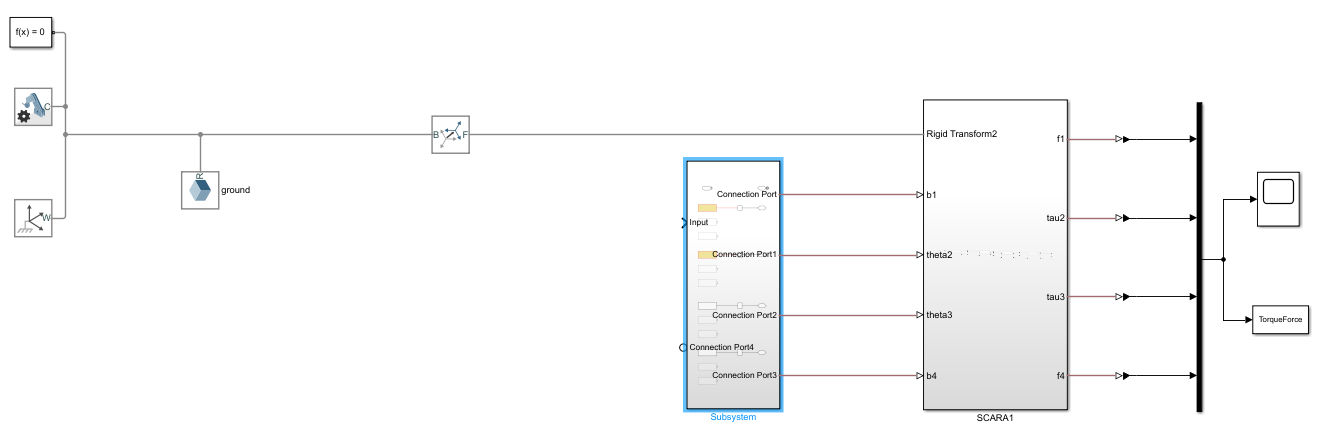
\includegraphics[width=0.5\textwidth]{figures/simulink.png}}
    \caption{An overview of the provided simulink environment}
    \label{fig:simulink}
\end{figure}

\section{Results}
\begin{figure}[htbp]
    \centerline{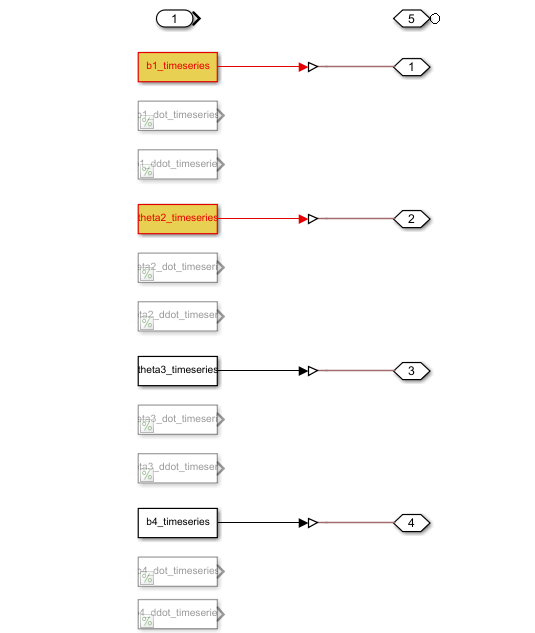
\includegraphics[width=0.48\textwidth]{figures/subsystem.png}}
    \caption{Modified inputs defined as subsystem added to the simulink file}
    \label{fig:sub}
\end{figure}

\begin{figure}[htbp]
    \centerline{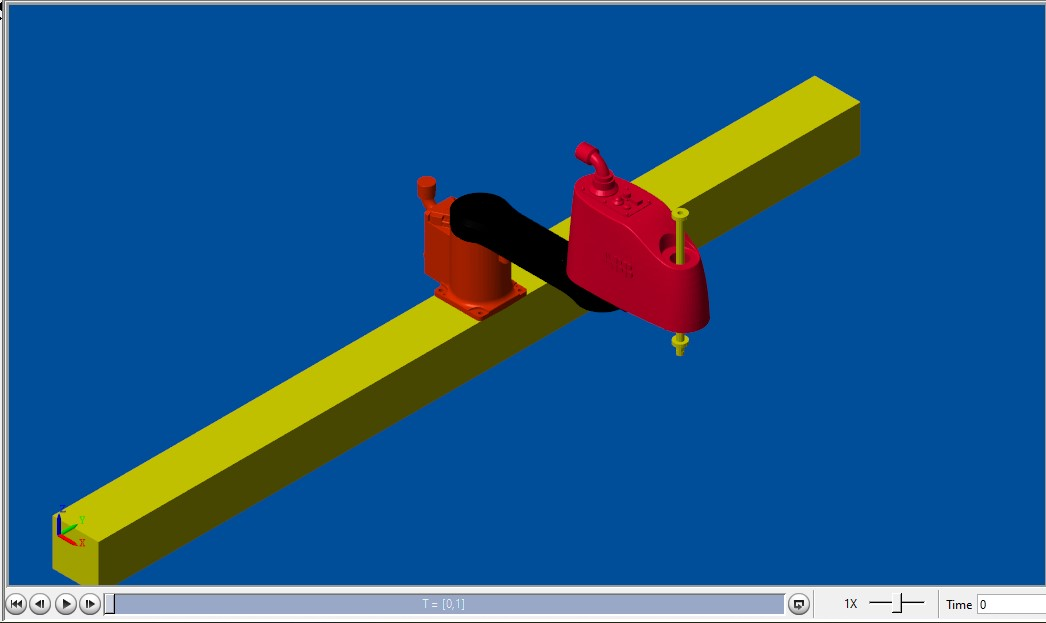
\includegraphics[width=0.45\textwidth]{figures/initial.jpg}}
    \centerline{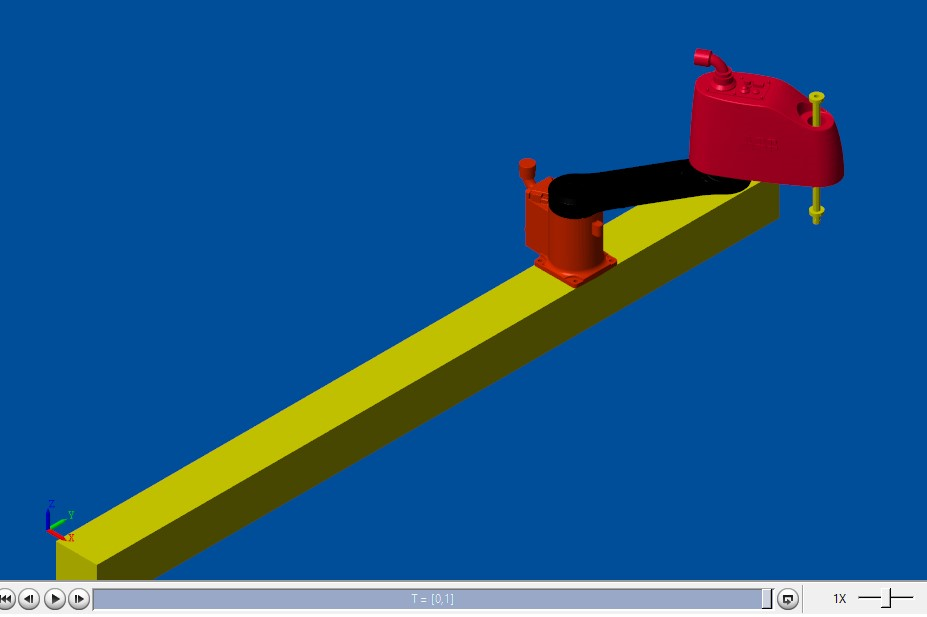
\includegraphics[width=0.45\textwidth]{figures/final.jpg}}
    \caption{Initial and final condition of the robot in the simulation}
    \label{fig:simulation}
\end{figure}

\begin{figure}[htbp]
    \centerline{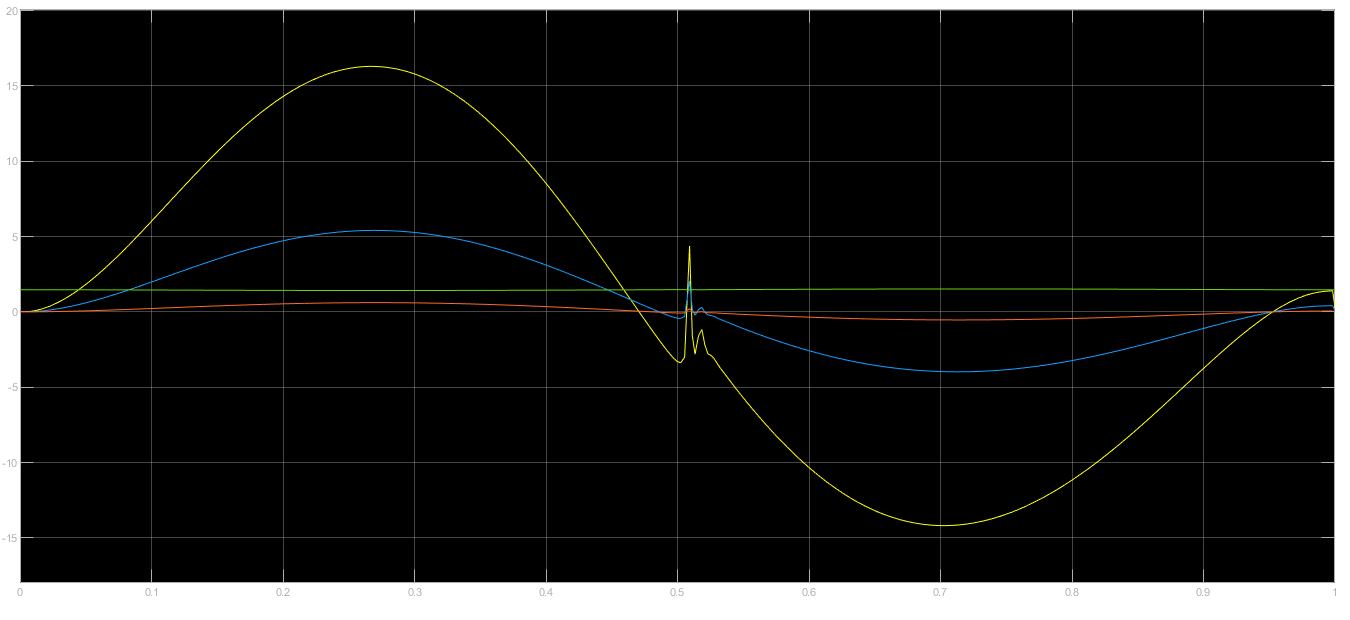
\includegraphics[width=0.5\textwidth]{figures/simulinkResult.png}}
    \caption{Overall result of the simulation on the joint forces and torques}
    \label{fig:sim_res}
\end{figure}

\begin{figure}[htbp]
    \centerline{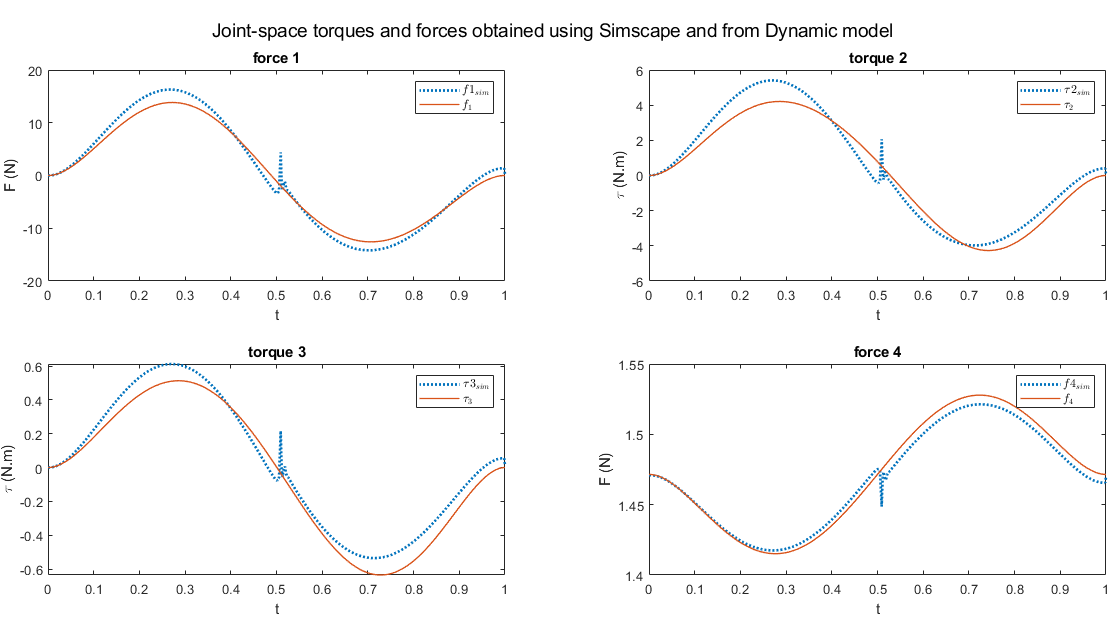
\includegraphics[width=0.5\textwidth]{figures/comparison.png}}
    \caption{Comparison of the simulation and analytical results in dynamic modeling of the SCARA robot under review}
    \label{fig:comparison}
\end{figure}
\vspace{10px}

\section{Conclusion}
\textbf{
    SCARA robots offer valuable advantages in manufacturing and assembly tasks due to their speed, precision, and cost-effectiveness. However, their limited range of motion restricts their suitability for certain applications. In conclusion, this report has delved into the \textit{kinematics} and \textit{dynamics} of a specific SCARA robot, deriving its D-H parameters, solving its Forward and Inverse kinematic problem, finding its Jacobian, achieving its dynamic model and verifying the results with MATLAB \textit{Simscape} simulations.
}
\vspace{10px}

\begin{thebibliography}{00}
    \bibitem{b1} J. Angeles, ``Fundamentals of Robotic Mechanical Systems'', Theory, Methods, and Algorithms, 4th edition, Springer.

    \bibitem{b2} J. J. Craig, ``Introduction to Robotics'', 3d edition, Pearson Education, Inc.

    \bibitem{b3} Wikipedia, 2023, ``SCARA'', Wikimedia Foundation, Last modified July 4, 2023. \url{https://en.wikipedia.org/wiki/SCARA}.

    \bibitem{b4} M. Kazim, J. Hong, M. Kim, K. K. Kim, (2023). ``Recent advances in path integral control for trajectory optimization: An overview in theoretical and algorithmic perspectives''. Annual Reviews in Control, 57, 100931. [Online]. Available: \url{https://doi.org/10.1016/j.arcontrol.2023.100931}

    \bibitem{b5} B. Nadir, O. Mohammed, N. Minh-Tuan, et al. ``Optimal trajectory generation method to find a smooth robot joint trajectory based on multiquadric radial basis functions''. Int J Adv Manuf Technol 120, 297-312 (2022). [Online]. Available: \url{https://doi.org/10.1007/s00170-022-08696-1}
\end{thebibliography}

\vspace{30px}


\end{document}
